\documentclass[letterpaper,11pt]{article}
\oddsidemargin -1.0cm \textwidth 17.5cm

\usepackage[utf8]{inputenc}
\usepackage[activeacute,spanish, es-lcroman]{babel}
\decimalpoint
\usepackage{amsfonts,setspace}
\usepackage{amsmath}
\usepackage{amssymb, amsmath, amsthm}
\usepackage{comment}
\usepackage{float}
\usepackage{amssymb}
\usepackage{dsfont}
\usepackage{anysize}
\usepackage{multicol}
\usepackage{enumerate}
\usepackage{graphicx}
\usepackage[left=1.5cm,top=2cm,right=1.5cm, bottom=1.7cm]{geometry}
\setlength\headheight{1.5em} 
\usepackage{fancyhdr}
\usepackage{multicol}
\usepackage{hyperref}
\usepackage{wrapfig}
\usepackage{subcaption}
\usepackage{siunitx}
\usepackage{cancel}
\usepackage{mdwlist}
\usepackage{svg}
\pagestyle{fancy}
\fancyhf{}
\renewcommand{\labelenumi}{\normalsize\bfseries P\arabic{enumi}.}
\renewcommand{\labelenumii}{\normalsize\bfseries (\alph{enumii})}
\renewcommand{\labelenumiii}{\normalsize\bfseries \roman{enumiii})}


\begin{document}

\fancyhead[L]{\itshape{Facultad de Ciencias F\'isicas y Matem\'aticas}}
\fancyhead[R]{\itshape{Universidad de Chile}}
\rfoot[]{pág. \thepage}

\begin{minipage}{11.5cm}
    \begin{flushleft}
        \hspace*{-0.6cm}\textbf{FI1000 Introducción a la Física Clásica}\\
        \hspace*{-0.6cm}\textbf{Tutor:} Alejandro Cartes
    \end{flushleft}
\end{minipage}

\begin{picture}(2,3)
    \put(366, -10){\includegraphics[scale=0.9]{2020-1/Imágenes/logo/dfi-fcfm.pdf}}
\end{picture}

\begin{center}
	\LARGE\textbf{Recopilatorio de Problemas}
\end{center}

\vspace{-1cm}

\section*{Trigonometría}

\begin{enumerate}\setlength{\itemsep}{0.4cm}

\item Dos observadores $A$ y $B$ miden ángulos de elevación de un avión que los sobrevuela a una altura constante. En cierto instante los ángulos medidos por $A$ y $B$ son $\alpha = 60^{\circ}$ y $\beta = 40^{\circ}$, respectivamente. La separación entre $A$ y  $B$ es $D = \SI{1}{\km}$. ¿A qué altura vuela el avión?

\begin{figure}[H]
    \centering
    \includegraphics[width=0.35\linewidth]{2021-1/Imagenes/aux0/avion.pdf}
\end{figure}


\item Una tortuga se encuentra al pie de un cerro cuya inclinación es $\gamma$. Desde cierta posición avista, con un ángulo de elevación $\alpha$ respecto al piso, a su compañera tortuga que se encuentra en la punta de un poste vertical ubicado en la cima del cerro. Luego, la tortuga avanza una distancia $d$ en dirección al poste. En este lugar avista a su compañera con un ángulo de elevación $\beta$. Encuentre la altura $h$ del poste en el que se encuentra la compañera tortuga. Analice el caso $\gamma\rightarrow 0$

\begin{figure}[H]
    \centering
        \centering
        \svgpath{2021-2/img/aux1}
        \includesvg[width=0.4\linewidth]{tortugas.svg}
\end{figure}

\item Una persona ubicada en el punto $P$ (ver Figura P2) observa dos montañas, una a la izquierda y otra a la derecha. Sean $\alpha$ y $\beta$ los ángulos de elevación de estas montañas. Si la montaña de la izquierda tiene una altura $h$ y la separación entre las proyecciones de las cimas sobre el nivel de la superficie terrestre es $D$, calcule la altura del otro monte. 


\begin{figure}[H]
    \centering
    \includegraphics[width=0.4\linewidth]{2021-1/Imagenes/aux0/mountain.pdf}
\end{figure}


\item Considere la construcción de la figura, determine:

\begin{multicols}{2}
    \begin{figure}[H]
        \centering
        \includesvg[width=0.55\linewidth]{2022-1/img/aux0/sumaangulos.svg}
    \end{figure}
    \columnbreak
    \begin{enumerate}
        \item Los segmentos $\overline{EA}$, $\overline{ED}$, $\overline{DF}$, $\overline{OD}$ y $\overline{DB}$.
        Concluya que: $$\sin\left(\alpha+\beta\right)=\cos\alpha\sin\beta+\sin\alpha\cos\beta$$
        \item Los segmentos $\overline{OA}$, $\overline{OB}$ y $\overline{EF}$.
        Concluya que: $$\cos\left(\alpha+\beta\right)=\cos\alpha\cos\beta-\sin\alpha\sin\beta$$
    \end{enumerate}
\end{multicols}

\item Un terraplén de ferrocarril se levanta sobre un plano horizontal, y se requiere encontrar la distancia desde un punto A de dicho plano a un punto B de la parte superior del terraplén. Se escoge un punto C en el pie del terraplén (que esté en el mismo plano vertical que A y B), y se miden las distancias $AC$, $AB$ y el ángulo $\alpha = \angle BAC$. Si $AC = \SI{14}{\m}$, $BC = \SI{25}{\m}$ y $\alpha = 21^{\circ}$, calcular la medida del lado AB.


 \begin{figure}[H]
    \centering
     \includegraphics[height=5cm]{2022-2/Imagenes/t1p2.jpg}
 \end{figure}

 \item Demuestre las siguientes relaciones trigonométricas:
    {
    \begin{multicols}{2}
        \begin{enumerate}
        \item $\sin^2\alpha = \cfrac{1 - \cos{(2\alpha)}}{2}$
        
        \item $\tan^2\alpha + 1 = sec^2\alpha$
        
        \columnbreak
        
        \item $\sin\alpha + \sin\beta = 2\sin{\left(\cfrac{\alpha+\beta}{2}\right)}\cos{\left(\cfrac{\alpha-\beta}{2}\right)}$
        
        \item $\cos\alpha+\cos\beta = 2\cos{\left(\cfrac{\alpha+\beta}{2}\right)}\cos{\left(\cfrac{\alpha-\beta}{2}\right)}$
    \end{enumerate}
    \end{multicols}
    }

\item Demuestre el teorema del seno y del coseno para un triángulo obtusángulo\\
\textbf{\textit{Hint:}} forme un triángulo rectángulo

\begin{figure}[H]
    \centering
    \begin{subfigure}[t]{0.6\textwidth}
        \centering
        \svgpath{2021-2/img/aux1}
        \includesvg[width=0.65\linewidth]{triangulo.svg}
    \end{subfigure}
    \hspace{1em}
    \begin{subfigure}[b]{0.30\textwidth}
        $\cdot$ Teo. seno:
        \begin{align*}
            \frac{\sin{\alpha}}{a}=\frac{\sin{\beta}}{b}=\frac{\sin{\gamma}}{c}
        \end{align*}
        
        $\cdot$ Teo. coseno:
        \begin{align*}
            a^2 &= b^2 + c^2 -2bc\cos{\alpha}\\
            b^2 &= a^2 + c^2 -2ac\cos{\beta}\\
            c^2 &= a^2 + b^2 -2ab\cos{\gamma}
        \end{align*}
    \end{subfigure}
\end{figure}

\item Demuestre el teorema del seno y del coseno para un triángulo acutángulo.\\
\textit{Hint:} forme triángulos rectángulos

\begin{figure}[H]
    \centering
    \begin{subfigure}[t]{0.4\textwidth}
        \centering
        \includegraphics[width=0.6\linewidth]{2021-1/Imagenes/aux0/acutangulo.pdf}
    \end{subfigure}
    \hspace{0.5cm}
    \begin{subfigure}[t]{0.4\textwidth}
        \vspace{-4cm}
        Teo. Seno:
        \begin{align*}
            \frac{\sin{\alpha}}{a} = \frac{\sin{\beta}}{b} = \frac{\sin{\gamma}}{c}
        \end{align*}
        
        Teo.Coseno
        \begin{align*}
            a^2 = b^2 + c^2 - 2bc \cos{\alpha}\\
            b^2 = a^2 + c^2 - 2ac \cos{\beta}\\
            c^2 = a^2 + b^2 - 2ab \cos{\gamma}
        \end{align*}
    \end{subfigure}
    \caption*{Figura P3}
\end{figure}

\item \href{https://www.geogebra.org/material/iframe/id/C6mhehH7/width/625/height/625/border/888888/sfsb/true/smb/false/stb/false/stbh/false/ai/false/asb/false/sri/false/rc/false/ld/false/sdz/false/ctl/false}{\textbf{Paralaje:}} Considere una estrella que se ubica perpendicularmente sobre el Sol. Encuentre una expresión para calcular la distancia Estrella-Sol utilizando el movimiento aparente de la estrella con respecto a las estrellas de fondo.
    \begin{figure}[H]
        \centering
        \includegraphics[scale=0.3]{2020-1/Imágenes/aux1/paralax.JPG}
    \end{figure}

\item Se desea hallar la altura de un globo, por lo cual se realizan las siguientes mediciones:

\begin{multicols}{2}
    \begin{figure}[H]
        \centering
        \includegraphics[width=0.4\linewidth]{2021-2/img/ejercicios/imagen_ej1.jpg}
    \end{figure}
    \columnbreak
    \begin{enumerate}
        \item Calcule la distancia entre el punto A y el globo.
        
        \item Calcule la distancia entre el punto B y el globo.
        
        \item Calcule la altura del globo.
        
        \item Exprese numéricamente la solución de los ítems anteriores, con una cantidad razonable de cifras decimales, sabiendo que $\alpha=90^{\circ}$, $\beta=75^{\circ}$, $\gamma=72^{\circ}$, $\delta=63^{\circ}$.  % cambié los º por \circ solo para quitar un warning uwu
    \end{enumerate}
    
    \textbf{\textit{Hint}}: Recuerde el Teo. del seno y del coseno
\end{multicols}

\end{enumerate}

\section*{Cinemática}

\begin{enumerate}\setlength{\itemsep}{0.4cm}

\item Una partícula se mueve a lo largo del eje $x$. En el tiempo $t=0$, la partícula se encuentra en $x=0$. La velocidad de la partícula cambia en función del tiempo como se muestra en el gráfico. Determine:

{
    \begin{multicols}{2}
        \begin{enumerate}
            
            \item La posición en $t=\SI{1}{\second}$
            
            \item La aceleración en $t=\SI{2}{\second}$
            
            \item La posición en $t=\SI{4}{\second}$
            
            \item La velocidad promedio entre $t=\SI{0}{\second}$ y $t=\SI{3}{\second}$
            
            \item La aceleración instantánea en $t=\SI{1}{\second}$ y en $t=\SI{3}{\second}$. ¿Es posible este movimiento físicamente?
        \end{enumerate}
        
        \columnbreak
        
        \begin{figure}[H]
            \centering
            \svgpath{2021-2/img/aux2}
            \includesvg[width=0.77\linewidth]{plot.svg}
        \end{figure}
    \end{multicols}
}

\item Dos vehículos parten de un mismo lugar y deben recorrer una distancia total $L$. El vehículo $A$ parte del reposo y recorrer la mitad del camino ($3L/4$) con aceleración constante $a_0$, y luego mantiene la velocidad final alcanzada, recorriendo la segunda mitad del camino con velocidad constante. Si el vehículo $B$ hace todo el recorrido a velocidad constante, determine a qué velocidad debe viajar para llegar al mismo instante que $A$ al final del trayecto.

\begin{figure}[H]
    \centering
    \svgpath{2021-2/img/aux2} 
    \includesvg[width=0.65\linewidth]{auto.svg}
\end{figure}


\item Dos vehículos parten de un mismo lugar y deben recorrer una distancia total $L$. El vehículo $A$ parte del reposo y recorrer la mitad del camino ($L/2$) con aceleración constante $a_0$, y luego mantiene la velocidad final alcanzada, recorriendo la segunda mitad del camino con velocidad constante. Si el vehículo $B$ hace todo el recorrido a velocidad constante, determine a qué velocidad debe viajar para llegar al mismo instante que $A$ al final del trayecto.

\begin{figure}[H]
    \centering
    \includegraphics[width = 0.6\linewidth]{2021-1/Imagenes/ejercicios/ej1.pdf}
    \caption{Vehículo A}
\end{figure}

\item Se tiene el siguiente gráfico que representa el movimiento de una partícula a lo largo de un eje rectilíneo:
    \begin{figure}[H]
        \centering
        \includegraphics[]{2020-1/Imágenes/ejercicios/Ejercicio_1_p1.png}
    \end{figure}
La escuela le pide a usted como experto en cinemática en 1-D que encuentre:
\begin{enumerate}
    \item La velocidad media, o promedio, en los siguientes intervalos de tiempo:
        \begin{enumerate}
            \item 0s a 2s
            \item 0s a 4s
            \item 2s a 4s
            \item 4s a 7s 
            \item 0s a 8s
        \end{enumerate}
    \item Calcule la velocidad instantánea a los:
        \begin{enumerate}
            \item t= 1 s
            \item t= 3 s
            \item t= 4,5 s
            \item t= 7,5 s
        \end{enumerate}
    \item ¿ Cuál es la velocidad instantánea en t=2,t=4,t=5,t=7? ¿Es la representación del gráfico físicamente posible ?
\end{enumerate}

\item
{
    \begin{multicols}{2}
        Una bola de acero se deja caer desde el techo de un edificio. Un observador parado frente a una ventana de altura $h$ nota que la bola cruza la ventana en $\tau$ segundos. La bola continua cayendo hasta chocar en forma completamente elástica con el piso (es decir, el módulo de su velocidad no cambia) y reaparece en la parte baja de la ventana $\tau_0$ segundos después. Demuestre que la altura del edificio está dada por la siguiente expresión:
        
        \centering{$H = \cfrac{g}{8}\left(\tau_0 + \tau + \cfrac{2h}{\tau g}\right)^2$}
        
        \columnbreak
        
        \begin{figure}[H]
            \centering
            \svgpath{2021-2/img/aux2}
            \includesvg[width=0.6\linewidth]{sus.svg}
        \end{figure}
        
    \end{multicols}
}

\item Dos autos (A y B) avanzan juntos por una calle, ambos con velocidad constante $v$. Cuando ambos autos están a distancia $L$ de un cruce se prende la luz amarilla del semáforo. El auto $A$ empieza a frenar con aceleración constante a modo de detenerse justo en el cruce. En tanto, el auto $B$ mantiene su velocidad. Transcurrido un tiempo $t_1$ desde que la luz cambió a amarilla, el semáforo cambia a rojo y entonces el auto $B$ empieza a frenar con aceleración constante para detenerse justo en el cruce (el auto $A$ sigue con aceleración que ya traía). Ambos autos se detienen exactamente en el mismo lugar.

\begin{enumerate}
    \item Muestre que es imposible que se detengan al mismo tiempo
    
    \item Grafique la posición y la velocidad de ambos autos en función del tiempo
\end{enumerate}

\item  \textbf{[\textit{C1 - Otoño 2022}]} Era la noche más oscura en Gotham, la luna comenzaba a esconderse en el horizonte
y el plan maestro de dos súper criminales iba a ser perpetrado. El plan consistía en asaltar
uno de los más grandes bancos de la ciudad, cuyas arcas estaban compuestas por grandes
fortunas de diferentes multimillonarios. Luego de perpetrar exitosamente el robo, el líder y
su cómplice se disponían a huir rumbo a un auto que los esperaba frente al asilo Arkham,
muchos metros más allá. En $t = 0$, el líder comenzó a correr con una velocidad de $v_l$ hacia la
derecha, mientras que su cómplice, mucho más lento por su falta de forma, a una velocidad
$v_c$ ($v_l > v_c$), también hacia la derecha. En un tiempo $t = T$, luego del aviso desesperado
de Jim Gordon, Batman aterriza heroicamente en el banco, con su capa flameante al viento
y rodilla al piso. Este se abalanza sobre los ladrones, partiendo desde el banco y desde el
reposo, con una aceleración constante $a_b$. Tras una vertiginosa persecución, Batman captura
fácilmente al cómplice, quien le suplicaba perdón, mientras que en ese mismo instante lanza
un grito ensordecedor al líder, ordenándole detenerse. Un fuerte escalofrío recorrió la espalda
del líder, afectando sus piernas, desacelerando con aceleración constante y deteniéndose luego
de avanzar una distancia $d_0$ desde que escuchó el grito.


\begin{enumerate}
    \item Represente, en un mismo gráfico, la posición de ambos malhechores y de Batman en
función del tiempo. Indique claramente cuál curva representa al líder de los malhechores,
cuál representa a su cómplice, y cuál representa a Batman.
    \item ¿A qué tiempo $t_2$ Batman logra alcanzar al cómplice, desde que los malhechores
comienzan a escapar?
    \item ¿A qué distancia del banco se encuentran Batman y cada uno de los malhechores
cuando Batman da alcance al cómplice?
    \item ¿Qué aceleración $a$ tiene el líder luego de que que Batman le ordena detenerse?
    \item ¿A qué tiempo $t_3$ se detuvo el líder, desde que comenzó su escapatoria?
\end{enumerate}

\item Michael Scott quiere probar si puede saltar en una cama elástica desde un edificio sin hacerse daño. Para aquello lanza una sandía con velocidad $v_1$ en un ángulo $\theta$ desde el techo de Dunder Mifflin Inc. Prontamente se da cuenta que la caída es sumamente peligrosa cuando observa la sandía salir eyectada con velocidad $v_2$ y ángulo $\alpha$ desde la cama elástica destruyendo el auto de Stanley. ($H,h_s,l_1$ y $h_a$ también son datos del problema)

\begin{figure}[H]
    \centering
        \centering
        \svgpath{2023-1/img/aux_2}
        \includesvg[width=0.8\textwidth]{Dunder_Mifflin.svg}
\end{figure}

\begin{enumerate}
    \item Encuentre el tiempo $t_1$ en el que la sandía toca la cama elástica y la velocidad $v_1$ con la que fue lanzada. 
    \item Despeje una expresión para $\alpha$ sabiendo que $v_2 = v(t_1)$ en función de los datos del problema. ($v(t_1)$ es la velocidad final del primer tramo)
    \item Finalmente, encuentre la distancia desde el impacto con el trampolín al auto de Stanley.
\end{enumerate}

\item Desde la azotea de un edificio de altura $H$ se lanza una pelota con una velocidad inicial $v$ en una dirección $\theta$ con respecto a la vertical. A una distancia horizontal $D$ del edifico se encuentra otro edificio de altura $h$ ($h < H$) y longitud $L$. Determine el rango de valores que puede tener la rapidez para que la pelota no caiga fuera de la azotea del segundo edificio.

\begin{figure}[H]
    \centering
    \includegraphics[width=0.4\linewidth]{2023-1/img/TD 1/edificios.png}
\end{figure}

\item 
\begin{multicols}{2}
Como se muestra en la Figura, se lanza un proyectil desde una ventana ubicada a una cierta altura. Dada una gran ventisca, existe aceleración horizontal $a_v$ que apunta en dirección al edificio, provocando que el proyectil se devuelva e ingrese a una ventana ubicada en un piso inferior. Si el proyectil se lanza con un ángulo $\alpha=45^{\circ}$ y rapidez $v_0$, determine:

\begin{enumerate}
    \item La distancia que separa a las ventanas por las cuales sale e ingresa el proyectil.
    
    \item La rapidez que tiene el proyectil al momento de ingresar por la ventana.
\end{enumerate}

\columnbreak

\begin{figure}[H]
    \centering
    \svgpath{2022-1/img/ejercicios}
    \includesvg[width=0.7\linewidth]{edificio.svg}
\end{figure}

\end{multicols}

\item Un viernes por la mañana, un papá quiere ir a dejar a su pequeño hijo al colegio. El papá se sube al auto y comienza a conducir con una rapidez constante $v_a$. Tras haber recorrido una distancia $L$ se percata que su hijo nunca se subió al auto, por lo que decide frenar con aceleración $a_{0}$ y retroceder hacia el punto de partida bajo la misma aceleración. Cuando vuelve a pasar por la distancia $L$, el padre acelera el automóvil de tal manera que pueda llegar con una velocidad nula hasta donde se encuentra su hijo, permitiéndole subir al auto.

\begin{enumerate}
    \item Determine la aceleración del último trayecto
    \item Determine cuánto tiempo estuvo el niño esperando
\end{enumerate}

\item 
\begin{multicols}{2}
    Una pelota es lanzada desde la base de una colina con un ángulo de lanzamiento $\alpha$ con respecto a la horizontal y una velocidad inicial $v_0$. Si La colina tiene un ángulo de elevación $\delta$, determine la distancia horizontal que la pelota recorre a lo largo de la colina.

    \columnbreak
    
    \begin{figure}[H]
        \centering
        \includegraphics[width=0.8\linewidth]{2023-1/img/TD 2/plano.png}
    \end{figure}
\end{multicols}


\item En el gráfico adjunto se representa la velocidad en función del tiempo para dos móviles, A y B, desplazándose a lo largo de un mismo trayecto rectilíneo. Se sabe además que cuando A alcanza la misma velocidad que B, ambos móviles se encuentran uno junto al otro. Determine la ubicación inicial de B si la posición inicial de A es A(t = 0) = 25 m.
    \begin{figure}[H]
        \centering
        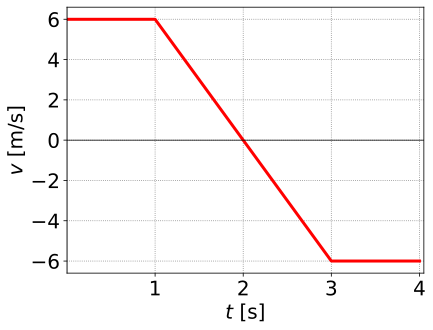
\includegraphics[scale=0.3]{2020-1/Imágenes/aux2/plot.png}
    \end{figure}
\item Se tiene el siguiente gráfico que esquematiza el movimiento de una partícula:
    \begin{figure}[H]
        \centering
        \includegraphics[scale=0.6]{2020-1/Imágenes/aux2/grafo.png}
    \end{figure}

\begin{enumerate}
    \item Calcule la velocidad media entre los puntos:
        \begin{enumerate}
            \item A-B
            \item A-C
            \item D-E
        \end{enumerate}
    \item Calcule la velocidad instantánea a los:
        \begin{enumerate}
            \item 3,5 seg.
            \item 2 seg.
            \item 6,8 seg.
        \end{enumerate}
\end{enumerate}
 \item Dos partículas A y B se encuentran separadas sobre un trayecto rectilíneo, estas se encuentran en $x_a$ y $x_b$, con $x_a<x_b$. En t=0 comienzan a moverse una hacia la otra con velocidades $v_a$ y $v_b$ respectivamente. Determine el tiempo y la posición de choque. 

\item Una bola se deja caer desde una altura h. Al mismo tiempo, un carro que se encuentra a una distancia horizontal $x_c$ comienza a moverse con velocidad $v_c$ hacia la bola. 
Determine la altura h tal que la bolita caiga dentro del carro. 

\item Un cohete se dispara verticalmente, subiendo con una aceleración constante $a_0$ respecto a la plataforma de lanzamiento durante un tiempo $\tau$. En ese momento se agota su combustible y continua moviéndose bajo la acción de la aceleración de gravedad.
    \begin{enumerate}
        \item ¿Cuál es la máxima altura que alcanza?
        \item ¿Cuál es el tiempo transcurrido desde que despega hasta volver a caer sobre la plataforma?
    \end{enumerate}
    
\item Un volcán eyecta lava y rocas desde su cráter. Suponga que una roca es eyectada con una velocidad inicial de $v_0 = $ \SI{25}{\m/\s} a un ángulo de $\theta = $ $35^{\circ}$ con respecto a la horizontal como lo muestra la figura. La roca impacta el suelo a una altura de $h = $ \SI{20}{\m} por debajo del nivel que fue lanzada.
    \begin{enumerate}
        \item Calcule el tiempo total de vuelo de la roca
        
        \item Calcule la magnitud del vector velocidad de la roca al impactar el suelo
    \end{enumerate}

\begin{figure}[H]
    \centering
    \includegraphics[width=0.5\linewidth]{2021-1/Imagenes/aux2/volcan.jpg}
    \caption*{Figura P2}
\end{figure}

\item Un cohete viaja verticalmente gracias a sus motores con una aceleración conocida $a_0$ hacia arriba, partiendo con velocidad nula. Al mismo instante en que parte el cohete y desde el mismo nivel, se dispara un proyectil con la intención de destruirlo en el aire. La separación horizontal cuando ambos objetos despegan es $L$, mientras que el ángulo inicial respecto a la horizontal del proyectil tiene un valor $\theta$. Calcule la rapidez inicial $v_0$ que posee el proyectil para que logre impactar el cohete

\begin{figure}[H]
    \centering
    \begin{subfigure}[t]{0.4\textwidth}
        \centering
        \includegraphics[width=0.8\linewidth]{2021-1/Imagenes/aux2/cohete-cannon.pdf}
    \end{subfigure}
\end{figure}

\item Si lanzo un objeto hacia arriba, desde el techo del costanera center, ubicado a 300 metros de altura con respecto al suelo, con una velocidad inicial $v_0$ = 35 m/s, ¿En cuanto tiempo llegaría ese objeto al suelo si consideramos condiciones ideales? (vacío) ¿Y si estuviéramos en la luna?\\
\textit{Hint: La gravedad en la luna es 1,62 m/s$^2$}

\begin{figure}[H]
        \centering
        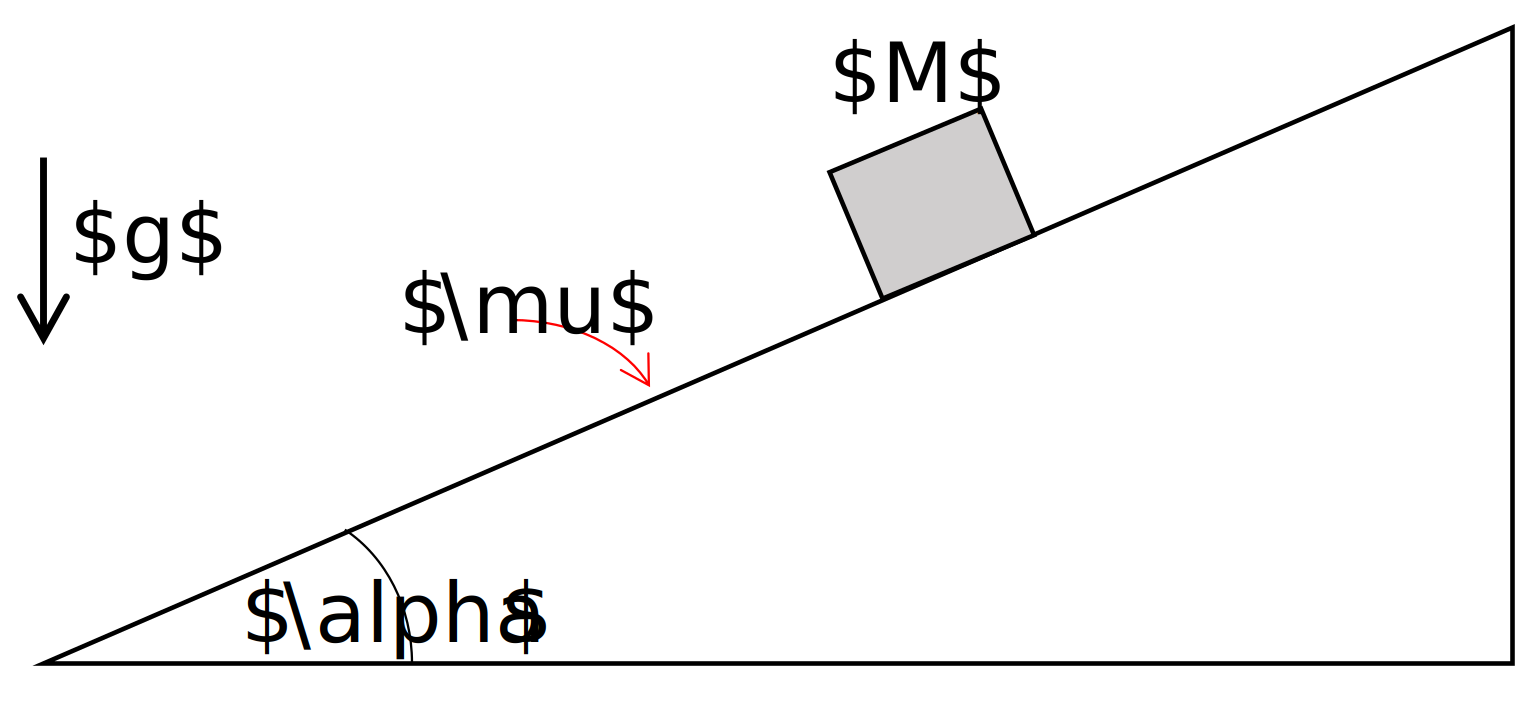
\includegraphics[scale=0.8]{2020-1/Imágenes/aux3/p1.png}
    \end{figure}


\item Un avión con cajas llenas de mascarillas e insumos médicos se mueve con extrema confidencialidad a lo largo de Chile repartiendo estos implementos, lo hace bajo tal nivel de secreto, que no puede aterrizar y solamente lanza los paquetes correspondientes a cada hospital desde la altura h a la que vuela. Si el avión vuela a una altura de 1500 m sobre el nivel del suelo y con una velocidad vo=360 km/hrs. ¿A que distancia horizontal L, con respecto al centro asistencial, debería lanzar los paquetes el avión?
    
   \begin{figure}[H]
        \centering
        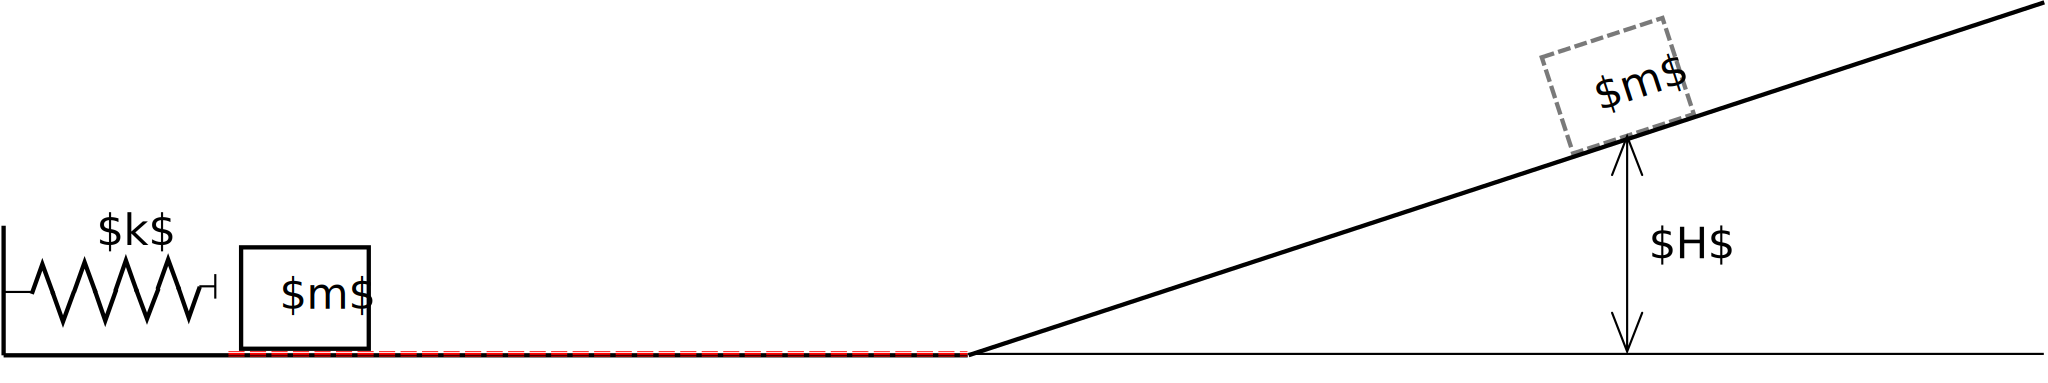
\includegraphics[scale=0.8]{2020-1/Imágenes/aux3/p2.png}
    \end{figure} 
    
\item  En presencia de la gravedad terrestre una pelota saltarina entra con rapidez $v_0$ por el techo de un pasillo de altura h. El ángulo de entrada de la pelota con respecto a la vertical es 
$\beta$ y tanto el techo como el piso del pasillo son lisos y horizontales. La pelota rebota elástica e indefinidamente entre el piso y el techo.

\begin{enumerate}
    \item Calcule el periodo T entre dos impactos consecutivos en el piso.
    
    \item En ausencia de gravedad, calcule el periodo T entre dos impactos consecutivos en el piso. Verifique que este es un caso particular de su respuesta (a)
    
    \item ¿Que distancia horizontal recorre la pelota entre dos impactos consecutivos con el suelo? (propuesto)
\end{enumerate}
    
\begin{figure}[H]
    \centering
    \begin{subfigure}[t]{0.4\linewidth}
        \centering
        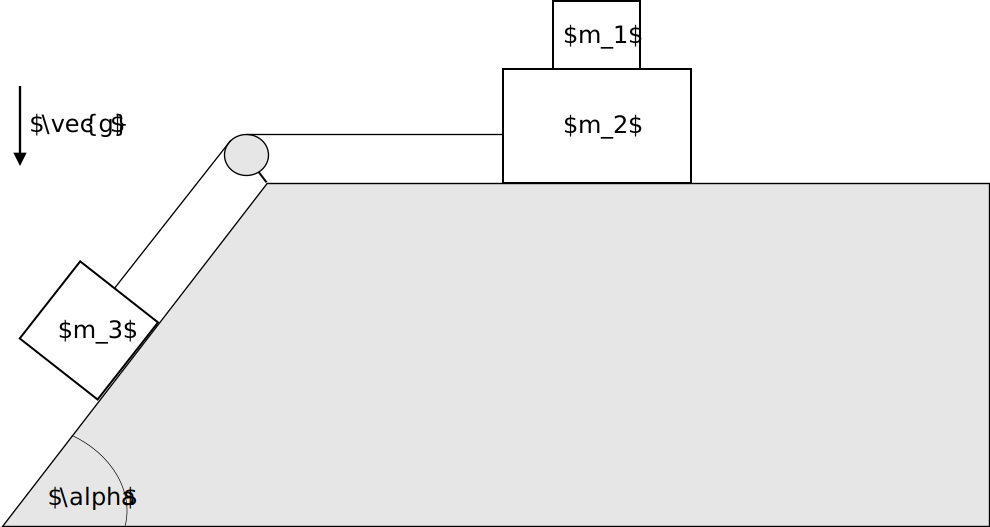
\includegraphics[width=0.9\linewidth]{2020-1/Imágenes/aux3/p3.png}
    \end{subfigure}
    \begin{subfigure}[t]{0.4\linewidth}
        \centering
         \includegraphics[width=0.9\linewidth]{2020-1/Imágenes/aux3/nota.png}
    \end{subfigure}
\end{figure} 

\item \textbf{[Propuesto]} Demuestre que para un proyectil disparado desde el suelo con un ángulo de lanzamiento \(\theta_0\) se cumple que:
\[\frac{H}{R} = \frac{1}{4}\tan{\theta_0}\]
donde $H$ es la altura máxima y $R$ es el alcance horizontal máximo

\item Se deja caer una piedra desde el borde superior de un pozo. Pasado un tiempo $T$ se escucha el
sonido del choque de la piedra con el agua. Determine la profundidad del pozo si la velocidad
del sonido es $u$ y el sonido se propaga como movimiento rectilíneo uniforme.

\begin{figure}[H]
    \centering
    \includegraphics[width=10cm]{2021-2/img/ejercicios/Pozo.pdf}
\end{figure}

\item Se lanzan dos proyectiles $A$ y $B$ de modo que tienen igual alcance horizontal $L$. $A$ se lanza horizontalmente desde una altura $h$, que es igual a la altura máxima que alcanza $B$ durante su vuelo.
{
    \begin{multicols}{2}
        \begin{enumerate}
            \item Calcule la razón entre los tiempos de vuelo de $A$ y $B$
            \item Calcule la razón entre las componentes horizontales de la velocidad de los proyectiles
            \item ¿Cuál es la rapidez de cada uno de ellos al llegar al suelo?
        \end{enumerate}
        
        \columnbreak
        
        \begin{figure}[H]
            \centering
            \svgpath{2022-1/img/aux2}
            \includesvg[width=1\linewidth]{dos lanzamientos.svg}
        \end{figure}
        
    \end{multicols}
}

\item Un cuerpo sube con velocidad constante $v_0$, en diagonal, de modo que su trayectoria forma un ángulo $\alpha$ respecto a la horizontal. Al mismo tiempo que el cuerpo comienza a subir, se lanza un proyectil con una velocidad inicial $\vec{v}_p$, formando un ángulo $\beta > \alpha$ con la horizontal.  Determine la distancia $D$ que debe separar el punto inferior del plano inclinado y el punto de lanzamiento del proyectil para que el cuerpo y el proyectil se encuentren.

\begin{figure}[H]
    \centering
    \begin{subfigure}[t]{1\textwidth}
        \centering
        \includegraphics[width=0.4\linewidth]{2022-1/img/aux2/colision.PNG}
    \end{subfigure}
\end{figure}


\item Determine la máxima distancia $\Delta$ que un objeto puede alejarse del borde de un peldaño para evitar ser alcanzado por los objetos lanzados con velocidad $v_0$ desde el punto $A$. La distancia desde $A$ al borde del peldaño es $L$ y la altura de este es $H$
\begin{figure}[H]
    \centering
    \begin{subfigure}[t]{1\textwidth}
        \centering
        \includegraphics[width=0.4\linewidth]{2022-1/img/aux2/peldanio.PNG}
    \end{subfigure}
\end{figure}

\item Una fila de soldados de largo $L$ marcha en líınea recta, uno detrás de otro. Un oficial recorre la columna, comenzando desde el último soldado, con rapidez constante $U$. En el instante que alcanza la cabeza de la columna, se devuelve con la misma rapidez, hasta que se encuentra con el último soldado de la columna. Durante este intervalo la columna de soldados ha permanecido en movimiento con rapidez constante $V$ y se ha desplazado una distancia $L$ desde el instante en que el oficial comenzó a adelantarse en la columna. De esta forma, el último soldado se encuentra en el lugar donde estuvo el primer soldado en el instante en que el oficial se dispuso a revisar la tropa.

\begin{enumerate}
    \item Dibuje un esquema de la situación
    \item Haga un gráfico con las posiciones del oficial y del último soldado de la fila en función del tiempo
    \item ¿Qué distancia total recorrió el oficial?
    \item Encuentre la razón entre los valores de $U$ y $V$
\end{enumerate}

\item Un automóvil viaja por la Ruta 5 Norte a exceso de velocidad, con rapidez constante $v_a$. El automóvil no se detiene en un punto de control policial, por lo que el carabinero ubicado en el control decide iniciar una persecución.

El carabinero tarda un tiempo $\tau$ en subirse a su vehículo, desde que pasa el automóvil por el control. Una vez en su vehículo, el carabinero acelera con magnitud constante $a_p$, hasta dar con el automóvil infractor.

\begin{enumerate}
    \item Represente cualitativamente, en un único gráfico, las posiciones del automóvil infractor y vehículo policial en función del tiempo.
    \item Determine la distancia entre del automóvil infractor y el vehículo policial, en el instante en que el policía comienza a acelerar.
    \item Determine el tiempo que tarda el policía en alcanzar al automóvil infractor, desde el momento en que el automóvil infractor pasa por el control policial.
    \item Determine la distancia total recorrida por el vehículo policial hasta dar con el vehículo infractor.
\end{enumerate}

\end{enumerate}
\subsection*{Mov. Circular}

\begin{enumerate}\setlength{\itemsep}{0.4cm}

\item Considere un eje vertical de largo $L$, en cuyos extremos hay dos discos sólidos provistos de ranuras. Las ranuras están desplazadas un cierto ángulo $\theta$ entre sí. El sistema gira con una velocidad angular $\omega$ constante. Calcule la altura $H$ por sobre el disco superior, desde la cual se debe soltar una bolita para que esta, en caída libre, pase por ambas ranuras.

\begin{figure}[H]
    \centering
    \includegraphics[scale = 0.4]{2020-1/Imágenes/aux4/vara_pelota.pdf}
\end{figure}

\item Un anillo muy pequeño se hace girar con velocidad angular constante $\omega$ a lo largo de una circunferencia vertical de radio $R$. La circunferencia está cortada en un punto determinado por un ángulo $\theta = 30^{\circ}$, como se señala en la figura. Al alcanzar este punto, el anillo se desprende y continua en caída libre.
    \begin{enumerate}
        \item Calcule el valor de la velocidad angular $\omega$ si el anillo, luego de desprenderse, toca a la circunferencia precisamente en su punto más bajo $P$
    
        \item Para el caso anterior indique la velocidad y la rapidez del anillo cuando cruza el diámetro de la circunferencia (eje $x$)
    \end{enumerate}
\begin{figure}[H]
    \centering
    \includegraphics[scale = 0.4]{2020-1/Imágenes/aux4/circ_pelota.pdf}
\end{figure}

\begin{multicols}{2}
\item Un anillo muy pequeño se hace girar con velocidad angular constante $\omega$ a lo largo de una circunferencia vertical de radio $R$. La circunferencia está cortada en un punto determinado por un ángulo $\theta$, como se señala en la figura. Al alcanzar este punto, el anillo se desprende y continua en caída libre.

    \begin{enumerate}
        \item Calcule el valor de la velocidad angular $\omega$ si el anillo, luego de desprenderse, toca a la circunferencia en el punto $P$ (ver figura)
    
        \item Para el caso anterior indique la velocidad y la rapidez del anillo cuando cruza el diámetro de la circunferencia (eje $x$)
    \end{enumerate}
    \columnbreak
    \begin{figure}[H]
        \centering
        \includegraphics[scale = 0.7]{2023-1/img/aux_3/anillo.png}
    \end{figure}
\end{multicols}

\item Cada lapsos de $\tau = 2.14 $ años la distancia entre la Tierra y Marte es mínima. Suponiendo órbitas circunferenciales, uniformes y coplanares, determine el periodo de órbita de Marte en el Sistema Solar. Examine su resultado para el caso $\tau$ muy grande e interprete.

\item Mientras gira, del punto más alto de una rueda de la fortuna se suelta un carro (vacío). Determine a qué distancia caerá el carro si la rueda tiene un radio $R$ y gira con velocidad angular constante $\omega$.\\
\textbf{\textit{Hint:}} En este problema deben usar lo aprendido en movimiento circular uniforme y lanzamiento de proyectil.
\begin{figure}[H]
    \centering
    \includegraphics[width=0.2\linewidth]{2020-1/Imágenes/ejercicios/rueda.PNG}
    \caption{Rueda de la fortuna lanza carros}
\end{figure}

\item Un mono se encuentra colgado de una rueda que gira horizontalmente con un periodo T, y que está a una altura H, como se indica en la figura. Además el eje sobre el cual gira la rueda esta en el borde de un plano inclinado, de ángulo $\theta$ con la horizontal. El mono se suelta justo cuando va pasando sobre el borde del plano inclinado tal que cae a una distancia D de ese punto. Determine el radio de la rueda
\begin{figure}[H]
        \centering
        \includegraphics[width=0.3\linewidth]{2020-1/Imágenes/aux5/fig1.pdf}/
\end{figure}

\item Dos tortugas comienzan una carrera desde el punto $A$. Una de ellas viaja en línea recta desde el punto $A$ hasta el punto $B$ con aceleración constante $a_0$, partiendo del reposo. La otra tortuga lo hace describiendo una semicircunferencia de radio $R$, moviéndose con rapidez constante. Si ambas llegan al mismo tiempo al punto $B$, ¿cuál es la velocidad angular $\omega$ de la segunda tortuga?
    
\begin{figure}[H]
    \centering
    \svgpath{2021-2/img/aux3}
    \begin{subfigure}[t]{1\textwidth}
        \centering
        \includesvg[width=0.4\linewidth]{carrera.svg}
    \end{subfigure}
\end{figure}

\item Un disco con un agujero a una distancia R del centro gira con velocidad angular $\omega$ respecto a un eje que pasa por su centro. Un proyectil se lanza desde el punto A en el instante en que el agujero se encuentra en dicha posición. Calcule la velocidad $\vec{v_0}$ y el ángulo $\theta$ de lanzamiento para que el proyectil pase por el agujero justo cuando éste se encuentra en el lado opuesto (punto B).

\begin{figure}[H]
    \centering
    \includegraphics[width=0.4\linewidth]{2021-2/img/ejercicios/imagen_ej3.png}
\end{figure}

\item 
\begin{multicols}{2}
     Imagine un mundo que transcurre sobre una plataforma circular de radio muy grande, que gira con velocidad angular $\Omega$ constante. En el entorno de la plataforma existe una aceleración de gravedad $\vec{g}$ constante. Una persona ubicada a una distancia $L$ del centro $O$, en reposo con respecto a la plataforma, lanza una moneda al aire en dirección vertical y con rapidez $v_0$ (respecto a la persona). 
    \columnbreak
    
    \begin{figure}[H]
        \centering
        \includegraphics[width = 0.8\linewidth]{2021-1/Imagenes/aux4/moneda-circulo.pdf}
    \end{figure}
\end{multicols}

Determine el tiempo que demora en caer la moneda al suelo y el lugar sobre la plataforma, con respecto a la persona, donde lo hace.
\textbf{\textit{Hint:}} Analice el lanzamiento de la moneda desde un observador ubicado en un sistema $S$ fijo con origen en $O$

\item Considere una persona en la superficie de la Tierra a una latitud $\lambda$. Sabiendo que el radio de la Tierra mide $R_{\oplus}=\SI{6370}{\km}$ y su periodo de rotación es de $\SI{24}{\hour}$, determine: rapidez angular, rapidez tangencial y aceleración centrípeta. ¿Qué sucede en los polos y en el ecuador?

\item 
\begin{multicols}{2}
    \begin{enumerate}
    
        \item Una piedra atada a una cuerda de largo $L$ se hace rotar de manera vertical. En cierto instante, la cuerda se corta como se muestra en la figura. Si la altura máxima alcanzada fue $H$, determine la rapidez angular $\omega$
    
        
        \item Si la cuerda se hubiera cortado en un ángulo $\alpha$ con respecto a la vertical. ¿Cómo hubiera sido la trayectoria? ¿Cuál sería la velocidad inicial? Si la altura máxima alcanzada hubiera seguido siendo $H$, ¿cómo cambia su respuesta de la parte (a)?
    
    \end{enumerate}

    \columnbreak

    \begin{figure}[H]
        \centering
        \includegraphics[width=0.45\linewidth]{2023-1/img/TD 2/piedra.png}
    \end{figure}
    
\end{multicols}


\section*{Dinámica}

\section*{Trabajo y Energía}

\section*{Sistema de N cuerpos}
\subsection*{Centro de Masa}

\section*{Estática}

\section*{Hidrostática}

\section*{Hidrodinámica}



% Para imágenes vectoriales -> el texto tiene que estar en LaTeX
% \begin{figure}[htbp]
%   \centering
%   \svgpath{../Imagenes/ejercicios}  -> .. irse pa'trás 
%   \includesvg{ej5.svg}
% \end{figure}

\end{enumerate}
\end{document}
